\documentclass[12pt]{article}
\usepackage{fullpage,graphicx,psfrag,amsmath,amsfonts,verbatim}
\usepackage[small,bf]{caption}

\input defs.tex

\bibliographystyle{alpha}

\title{Assignment 2 CME 241}
\author{Taylor Howell}

\begin{document}
\maketitle

\paragraph{1.}
The state space of Snakes and Ladders has 100 discrete states $\mathcal{S} = [1, 100]$. There is a single terminal state $\mathcal{T} = 100$. States $s_t \in [1, 95]$ have six possible next states $s_t$, each with equal probability of transition, $\mathcal{P}(S_{t+1} | S_t) = \frac{1}{6}$. Often, $s_{t+1}$ is simply the current state plus whatever number is rolled. However, in the cases where a snake or ladder exists the mapping is different. States $s_t \in [95, 100]$ have less possible next states (fewer for states that are near 100) with more probability of transitioning into the next state.

\paragraph{2.}
Fig. \ref{snakes_and_ladders} shows a histogram with the number of transitions required to complete Snakes and Ladders over 100 trials. See $\texttt{snakes\_and\_ladders.py}$. 
\begin{figure}[h]
	\centering
	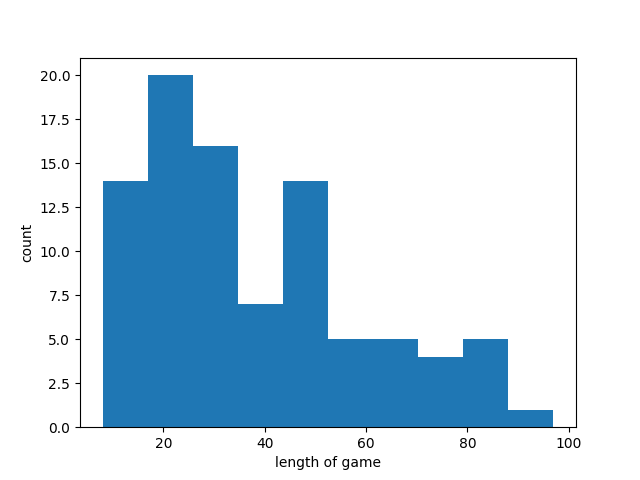
\includegraphics[width=.5\textwidth]{snakes_and_ladders_length_histogram.png}
	\caption{Histogram showing the number of transitions to complete Snakes and Ladders for 100 trials.}
	\label{snakes_and_ladders}
\end{figure}


\end{document}
